% 2013 重庆卷理科第 14 题：直角三角形外接圆与切线。
% ∠C=90°，∠A=60°，AB=20 为外接圆直径；CD 切圆于 C，BD⊥CD 于 D，BD 与圆交于 E。
% 图中取圆半径 3（即 10 按 0.3 缩放），C 在最下方，A 在左下，B 在右上，E 在 B、D 之间。
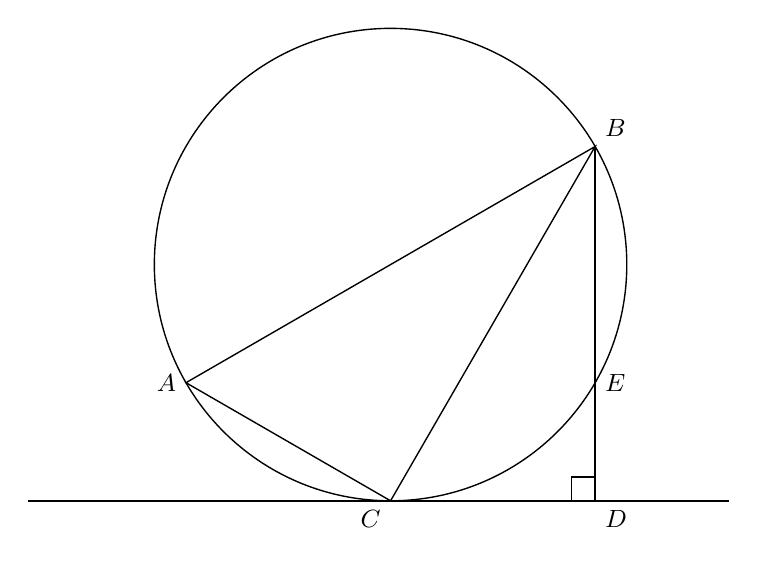
\begin{tikzpicture}[font=\small, line width=0.5pt, scale=1]
  \coordinate (O) at (0,0);
  \coordinate (C) at (0,-3);
  \coordinate (A) at (-2.5981,-1.5);
  \coordinate (B) at (2.5981,1.5);
  \coordinate (D) at (2.5981,-3);
  \coordinate (E) at (2.5981,-1.5);
  \draw (O) circle (3);
  % 切线 CD
  \draw (-4.6,-3) -- (4.3,-3);
  % 三角形与垂线
  \draw (A) -- (B) -- (C) -- cycle;
  \draw (B) -- (D);
  \draw (C) -- (D);
  % 直角标记（∠BCD 处，BC 与 CD 之间）
  \draw (2.5981,-2.7) -- (2.2981,-2.7) -- (2.2981,-3);
  \node[below left] at (C) {$C$};
  \node[left] at (A) {$A$};
  \node[above right] at (B) {$B$};
  \node[below right] at (D) {$D$};
  \node[right] at (E) {$E$};
\end{tikzpicture}
